\documentclass[aspectratio=169,11pt]{beamer}

\usetheme{Madrid}
\usecolortheme{default}
\setbeamertemplate{navigation symbols}{}
\setbeamertemplate{footline}[frame number]

\usepackage[utf8]{inputenc}
\usepackage[T1]{fontenc}
\usepackage[brazil]{babel}
\usepackage{booktabs}
\usepackage{graphicx}
\usepackage{amsmath,amssymb}

\graphicspath{{../ieee/figures/}{../classification/figures/}{../classification/figures/confusion/}}

\title{Classificação multiclasse de janelas de FBGs\\para demodulação de LPFG}
\subtitle{Trabalho Final --- Reconhecimento de Padrões}
\author{Jakson da Rocha Almeida}
\institute{Programa de Pós-Graduação em Engenharia Elétrica\\Universidade Federal de Juiz de Fora (UFJF)}
\date{}

\begin{document}

\begin{frame}
  \titlepage
\end{frame}

\begin{frame}{Roteiro}
  \tableofcontents
\end{frame}

\section{Motivação e problema}

\begin{frame}{Motivação}
  \begin{itemize}
    \item Sensores LPFG exigem, em geral, interrogação espectral cara.
    \item Alternativa: array de FBGs + aprendizado de máquina para estimar $\lambda_{res}$.
    \item No trabalho do Barino, a atenção sugere que \textbf{nem todas as FBGs importam igualmente}.
  \end{itemize}
  \vspace{0.6em}
  \textbf{Pergunta de RP:}\\
  a partir das potências das 13 FBGs, \emph{qual janela} de 4 FBGs contíguas é a relevante?
\end{frame}

\begin{frame}{Objetivo deste trabalho}
  \begin{block}{Parte 1 --- Classificação (foco)}
    Predizer a \textbf{classe} $s\in\{0,\ldots,9\}$ correspondente à janela\\
    $C_s=\{s,s+1,s+2,s+3\}$ (4 FBGs contíguas).
  \end{block}
  \begin{block}{Parte 2 --- Interrogação (contexto)}
    Estimar $\lambda_{res}$ (já feita no paper do Barino; não refeita aqui).
  \end{block}
  \vspace{0.4em}
  Entregas: artigo IEEEtran + apresentação (15~min).
\end{frame}

\begin{frame}{Formulação multiclasse (10 classes)}
  \begin{columns}[T]
    \begin{column}{0.52\textwidth}
      \textbf{Entrada} $\mathbf{x}\in\mathbb{R}^{13}$\\
      potências ópticas normalizadas.
      \vspace{0.5em}

      \textbf{Rótulo} $y=s\in\{0,\ldots,9\}$\\[0.3em]
      máscara top-4 por $|\lambda_{\mathrm{FBG}}-\lambda_{res}|$\\
      $\Rightarrow$ sempre janela contígua nos dados.
      \vspace{0.5em}

      \textbf{Predição:} $\hat{s}=\arg\max$ da classe\\
      (máscara implícita $=C_{\hat{s}}$).
    \end{column}
    \begin{column}{0.46\textwidth}
      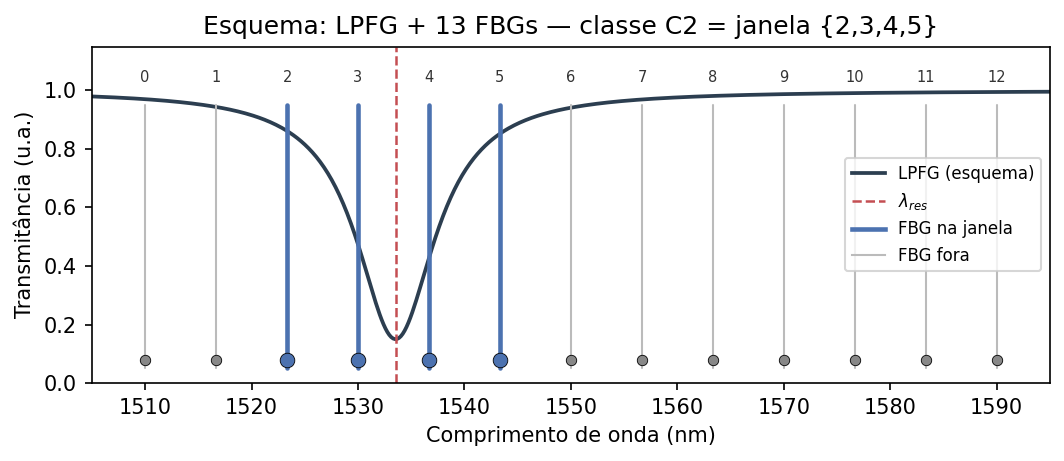
\includegraphics[width=\linewidth]{fig_schema_lpg_fbg.png}
    \end{column}
  \end{columns}
\end{frame}

\section{Dados e pré-processamento}

\begin{frame}{Dados}
  \begin{itemize}
    \item Fonte: \texttt{measured.dataset} (dados \textbf{reais}, autorizados).
    \item Bruto: 8200 $\rightarrow$ filtrado ($1515<\lambda_{res}<1585$): \textbf{7300}.
    \item Normalização: $X\leftarrow X-\min(X)$; $X\leftarrow X/\sum X$.
    \item \textbf{10 classes} presentes; desbalanceadas (ex.: $C_2{\approx}29\%$, $C_3{\approx}1{,}2\%$).
  \end{itemize}
\end{frame}

\begin{frame}{Pré-processamento}
  \begin{itemize}
    \item Filtro de faixa alinhado ao Barino.
    \item Rótulo: janela top-4 $\rightarrow$ classe $C_0,\ldots,C_9$.
    \item Observação: máscara 100\% contígua $\Rightarrow$ multiclasse é natural.
  \end{itemize}
\end{frame}

\section{Metodologia}

\begin{frame}{Protocolo de avaliação}
  \begin{itemize}
    \item Hold-out estratificado por \textbf{classe} (20\%): 1460 amostras.
    \item CV: StratifiedKFold 5 folds no desenvolvimento (5840).
    \item Nested CV para hiperparâmetros (scorer $=$ \textbf{acurácia}).
    \item Hold-out avaliado \emph{uma vez} após o tuning.
  \end{itemize}
\end{frame}

\begin{frame}{Classificadores}
  Seis métodos da disciplina (multiclasse nativo):
  \begin{columns}[T]
    \begin{column}{0.48\textwidth}
      \begin{itemize}
        \item kNN (+ scaler)
        \item SVM RBF
        \item MLP (+ scaler)
      \end{itemize}
    \end{column}
    \begin{column}{0.48\textwidth}
      \begin{itemize}
        \item Random Forest
        \item AdaBoost
        \item MQ / RidgeClassifier
      \end{itemize}
    \end{column}
  \end{columns}
  \vspace{0.8em}
  \textbf{Métricas:} acurácia, F1 weighted/macro, matriz $10\times 10$.
\end{frame}

\begin{frame}{Tuning (nested CV)}
  \begin{itemize}
    \item Consenso estável do SVM: $C{=}10$, $\gamma{=}0{,}1$ (todos os folds).
    \item Maior ganho do tuning: SVM acurácia $0{,}905\rightarrow 0{,}934$ (+0{,}029).
  \end{itemize}
\end{frame}

\section{Resultados}

\begin{frame}{Resultados --- CV (modelos afinados)}
  \begin{table}
    \centering
    \scriptsize
    \begin{tabular}{lccc}
      \toprule
      Método & Acurácia & F1 weight. & F1 macro \\
      \midrule
      \textbf{SVM} & $\mathbf{0{,}934\pm0{,}004}$ & 0{,}927 & 0{,}866 \\
      Random Forest & $0{,}929\pm0{,}003$ & 0{,}923 & 0{,}857 \\
      AdaBoost & $0{,}924\pm0{,}004$ & 0{,}923 & 0{,}871 \\
      MLP & $0{,}919\pm0{,}010$ & 0{,}908 & 0{,}819 \\
      kNN & $0{,}907\pm0{,}003$ & 0{,}901 & 0{,}830 \\
      MQ & $0{,}779\pm0{,}006$ & 0{,}736 & 0{,}580 \\
      \bottomrule
    \end{tabular}
  \end{table}
\end{frame}

\begin{frame}{Resultados --- hold-out}
  \begin{table}
    \centering
    \scriptsize
    \begin{tabular}{lccc}
      \toprule
      Método & Acurácia & F1 weight. & F1 macro \\
      \midrule
      \textbf{SVM} & $\mathbf{0{,}938}$ & 0{,}931 & 0{,}874 \\
      Random Forest & $\mathbf{0{,}938}$ & 0{,}932 & 0{,}878 \\
      MLP & 0{,}933 & 0{,}923 & 0{,}846 \\
      AdaBoost & 0{,}923 & 0{,}925 & 0{,}873 \\
      kNN & 0{,}919 & 0{,}911 & 0{,}824 \\
      MQ & 0{,}789 & 0{,}750 & 0{,}613 \\
      \bottomrule
    \end{tabular}
  \end{table}
  \vspace{0.4em}
  Ranking estável: \textbf{SVM} e \textbf{RF} lideram no hold-out.
\end{frame}

\begin{frame}{Exemplo: janela verdadeira vs prevista}
  \begin{center}
    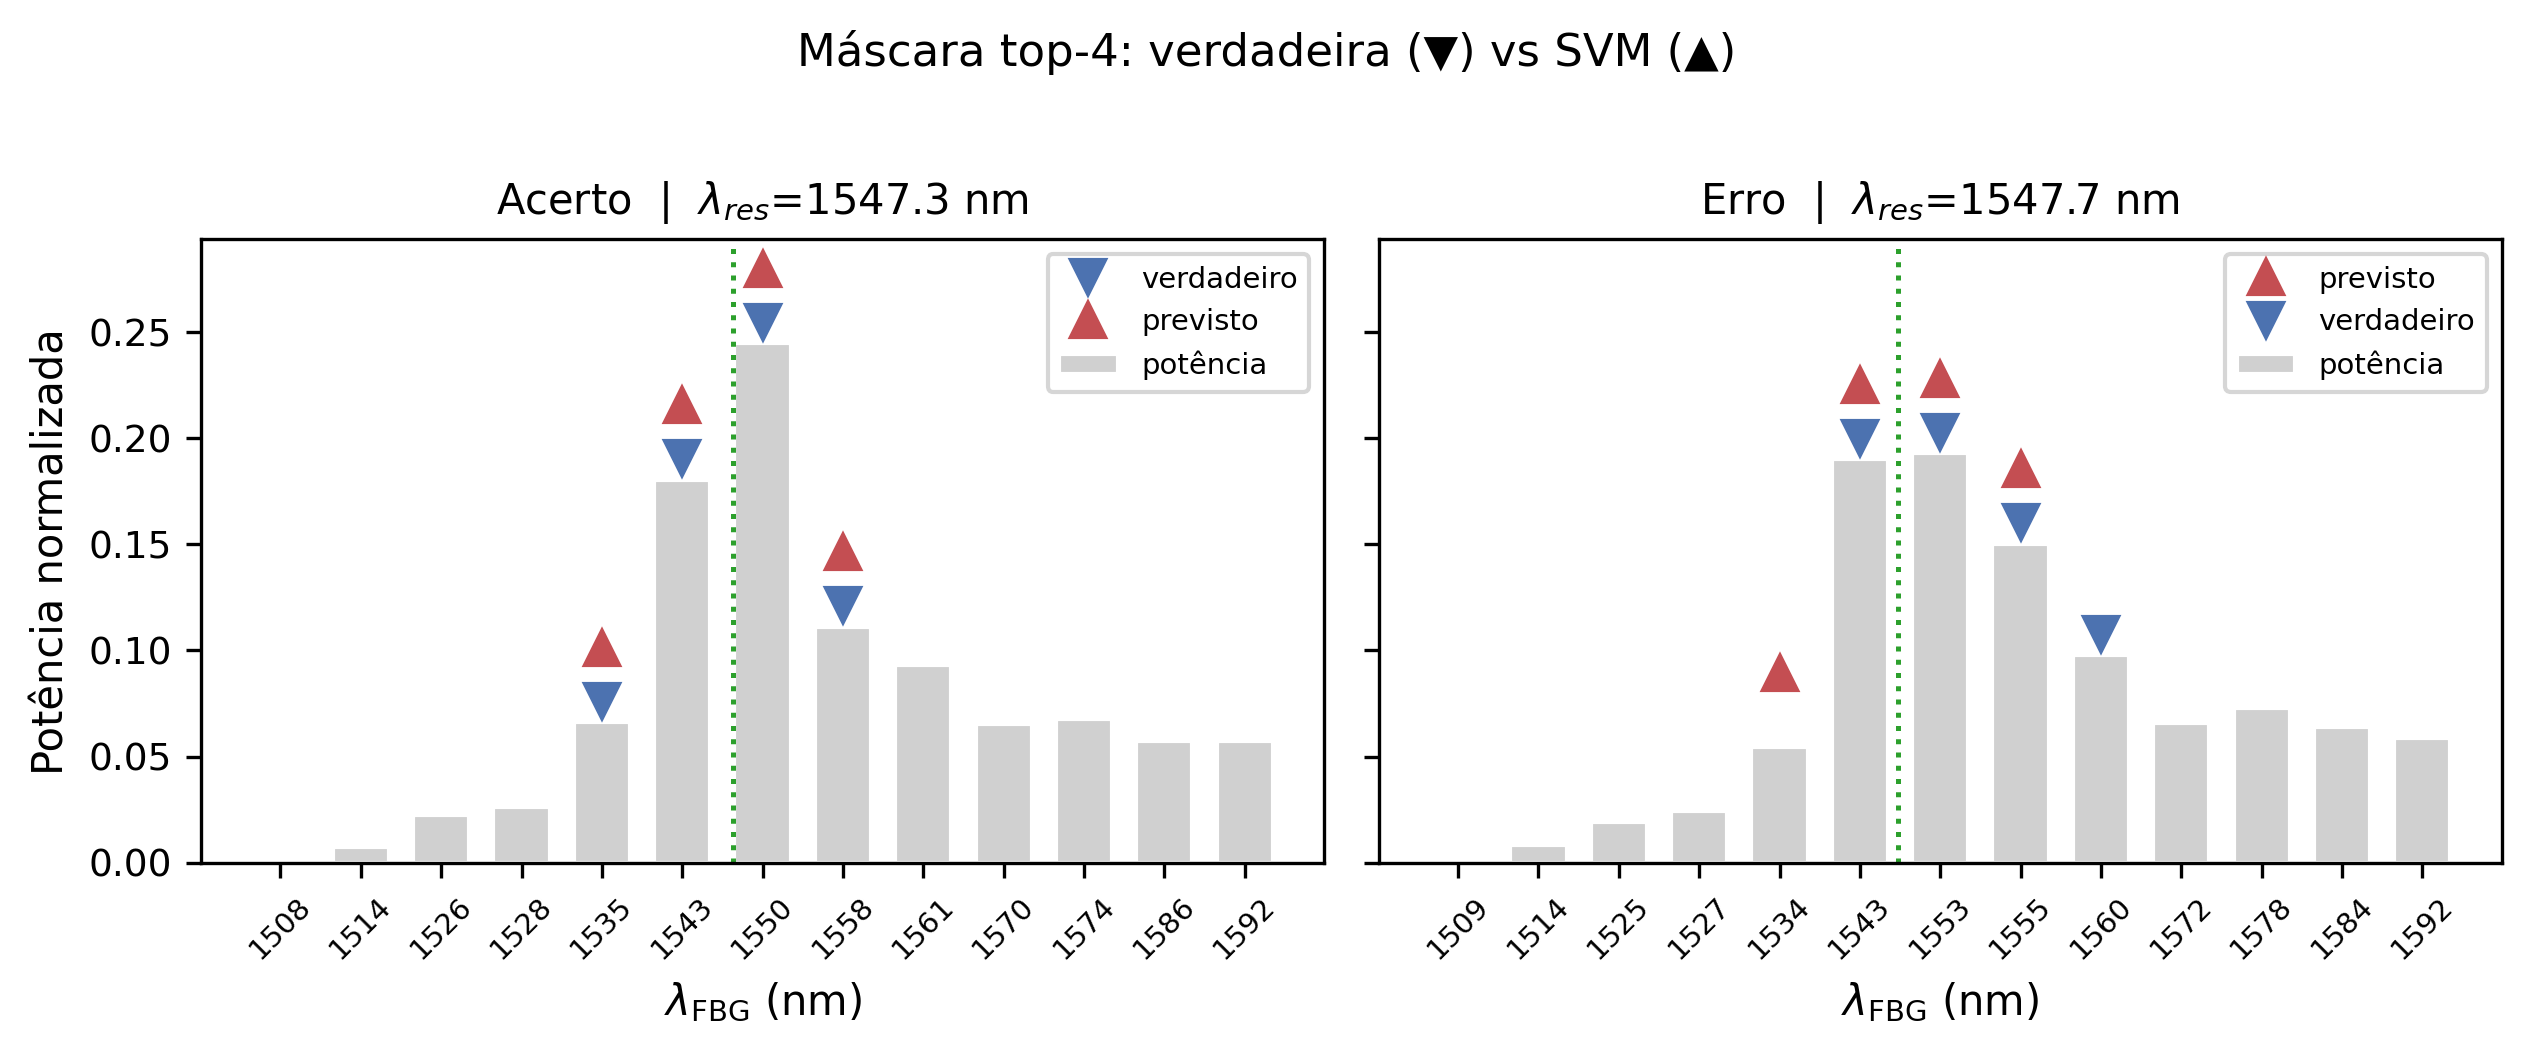
\includegraphics[width=0.85\linewidth]{fig_mask_true_vs_pred.png}
  \end{center}
\end{frame}

\begin{frame}{Análise: erros vs $\lambda_{res}$}
  \begin{itemize}
    \item Pior faixa do SVM: ${\approx}1548$--$1580$~nm (acurácia ${\approx}0{,}87$).
    \item Faixa $1531$--$1534$~nm: acurácia ${\approx}0{,}996$.
  \end{itemize}
  \begin{center}
    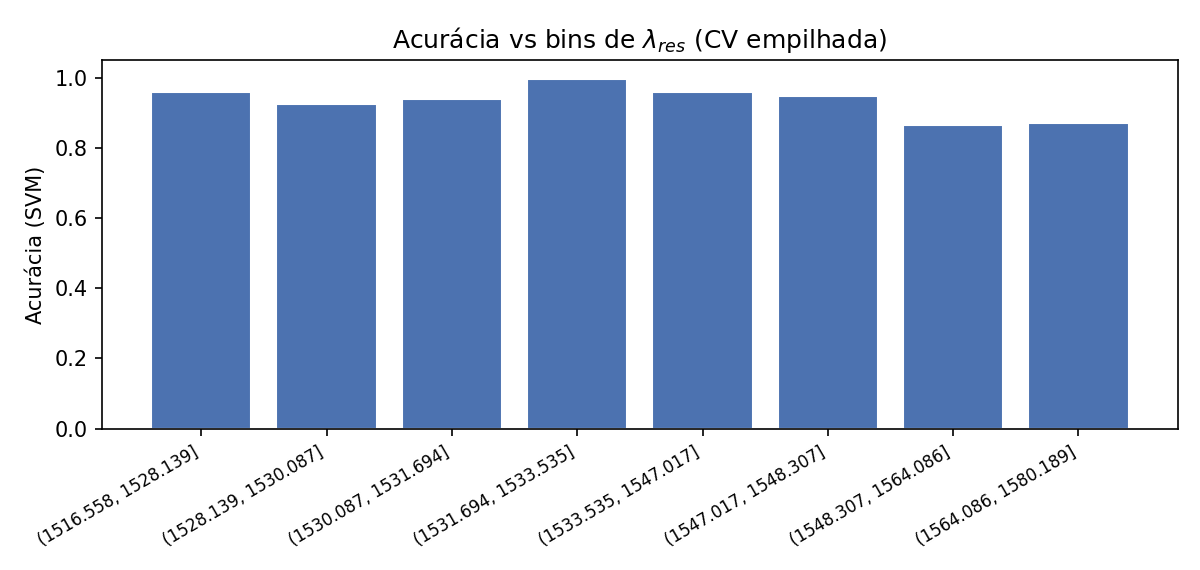
\includegraphics[width=0.72\linewidth]{fig_acc_vs_lambda.png}
  \end{center}
\end{frame}

\begin{frame}{Matrizes de confusão $10\times 10$ (1/2)}
  \begin{columns}[T,onlytextwidth]
    \begin{column}{0.32\textwidth}
      \centering\scriptsize SVM\\
      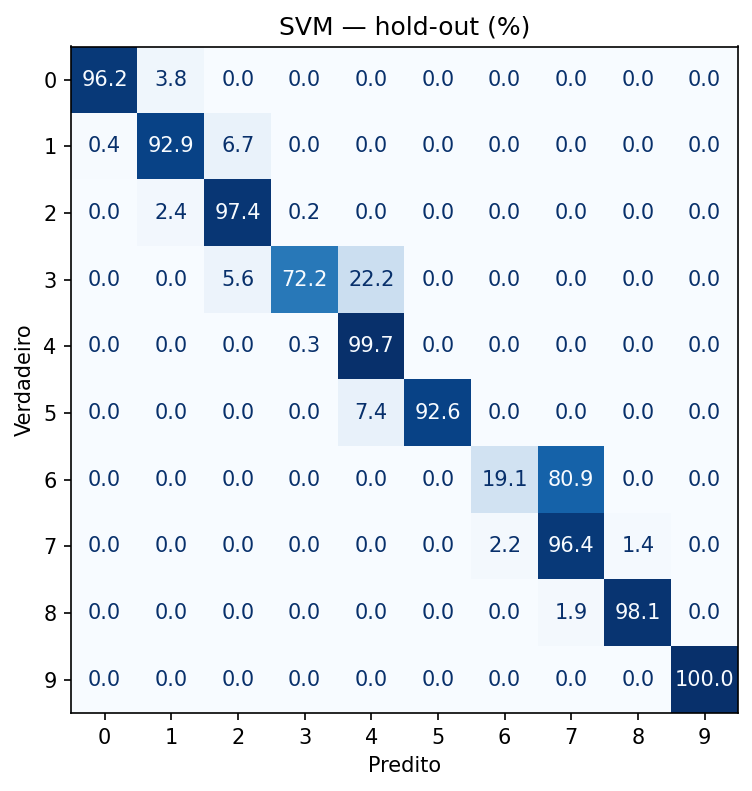
\includegraphics[width=\linewidth]{cm_agg_SVM_pct.png}
    \end{column}
    \begin{column}{0.32\textwidth}
      \centering\scriptsize Random Forest\\
      
\includegraphics[width=\linewidth]{cm_agg_RandomForest_pct.png}
    \end{column}
    \begin{column}{0.32\textwidth}
      \centering\scriptsize MLP\\
      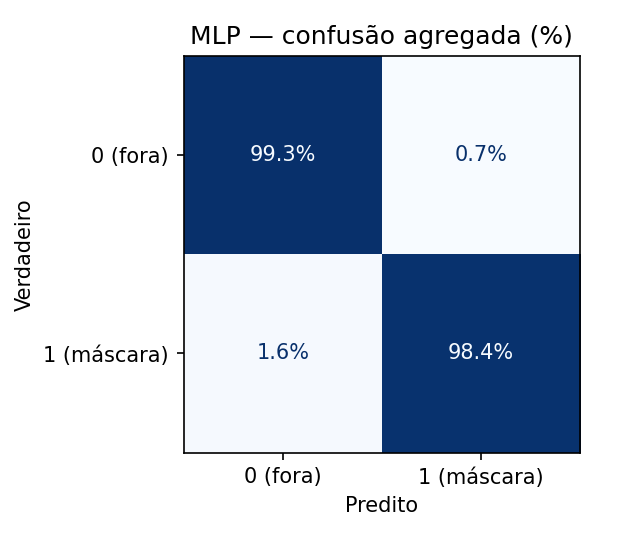
\includegraphics[width=\linewidth]{cm_agg_MLP_pct.png}
    \end{column}
  \end{columns}
\end{frame}

\begin{frame}{Matrizes de confusão $10\times 10$ (2/2)}
  \begin{columns}[T,onlytextwidth]
    \begin{column}{0.32\textwidth}
      \centering\scriptsize AdaBoost\\
      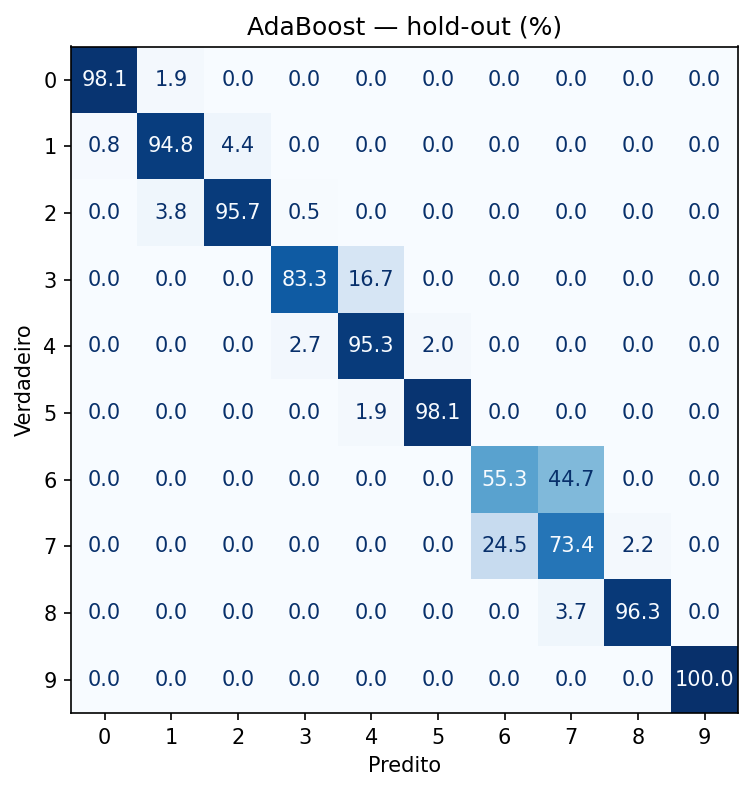
\includegraphics[width=\linewidth]{cm_agg_AdaBoost_pct.png}
    \end{column}
    \begin{column}{0.32\textwidth}
      \centering\scriptsize kNN\\
      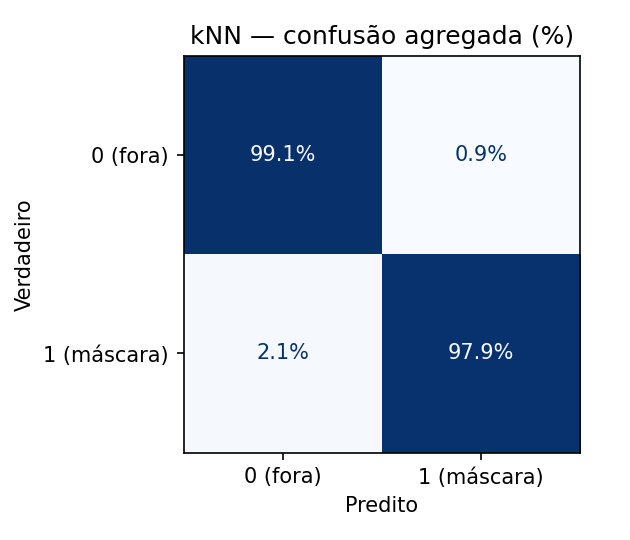
\includegraphics[width=\linewidth]{cm_agg_kNN_pct.png}
    \end{column}
    \begin{column}{0.32\textwidth}
      \centering\scriptsize MQ\\
      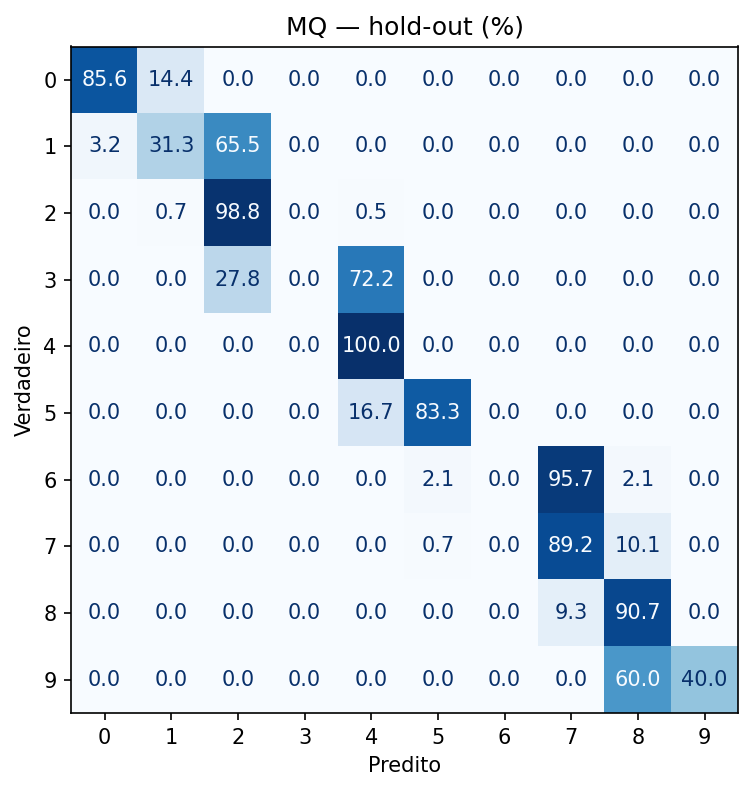
\includegraphics[width=\linewidth]{cm_agg_MQ_pct.png}
    \end{column}
  \end{columns}
\end{frame}

\begin{frame}{Ablation: $+$ posições Bragg}
  \begin{itemize}
    \item Melhora MLP/RF/MQ; quase neutro no SVM; \textbf{piora} o kNN ($-0{,}05$).
  \end{itemize}
\end{frame}

\section{Conclusões}

\begin{frame}{Conclusões}
  \begin{itemize}
    \item Problema de RP bem posto: \textbf{10 classes} de janelas contíguas.
    \item Métricas alinhadas à disciplina: acurácia + matriz de confusão.
    \item Melhores métodos: \textbf{SVM} e \textbf{Random Forest} (acurácia ${\approx}0{,}938$ no hold-out).
    \item Classes raras ($C_3$, $C_9$) são a limitação principal.
    \item Próximo passo: acoplar a janela à regressão de $\lambda_{res}$.
  \end{itemize}
\end{frame}

\begin{frame}{Agradecimentos}
  \begin{center}
    Agradecimento ao Dr.~Felipe Oliveira Barino\\
    pela autorização de uso dos dados e código.
    \vspace{1.2em}

    \textbf{Obrigado.}\\[0.5em]
    Perguntas?
  \end{center}
\end{frame}

\end{document}
